\documentclass[../../D1.tex]{subfiles}

\begin{document}

\subsection{Plan}

\begin{figure}[h]
    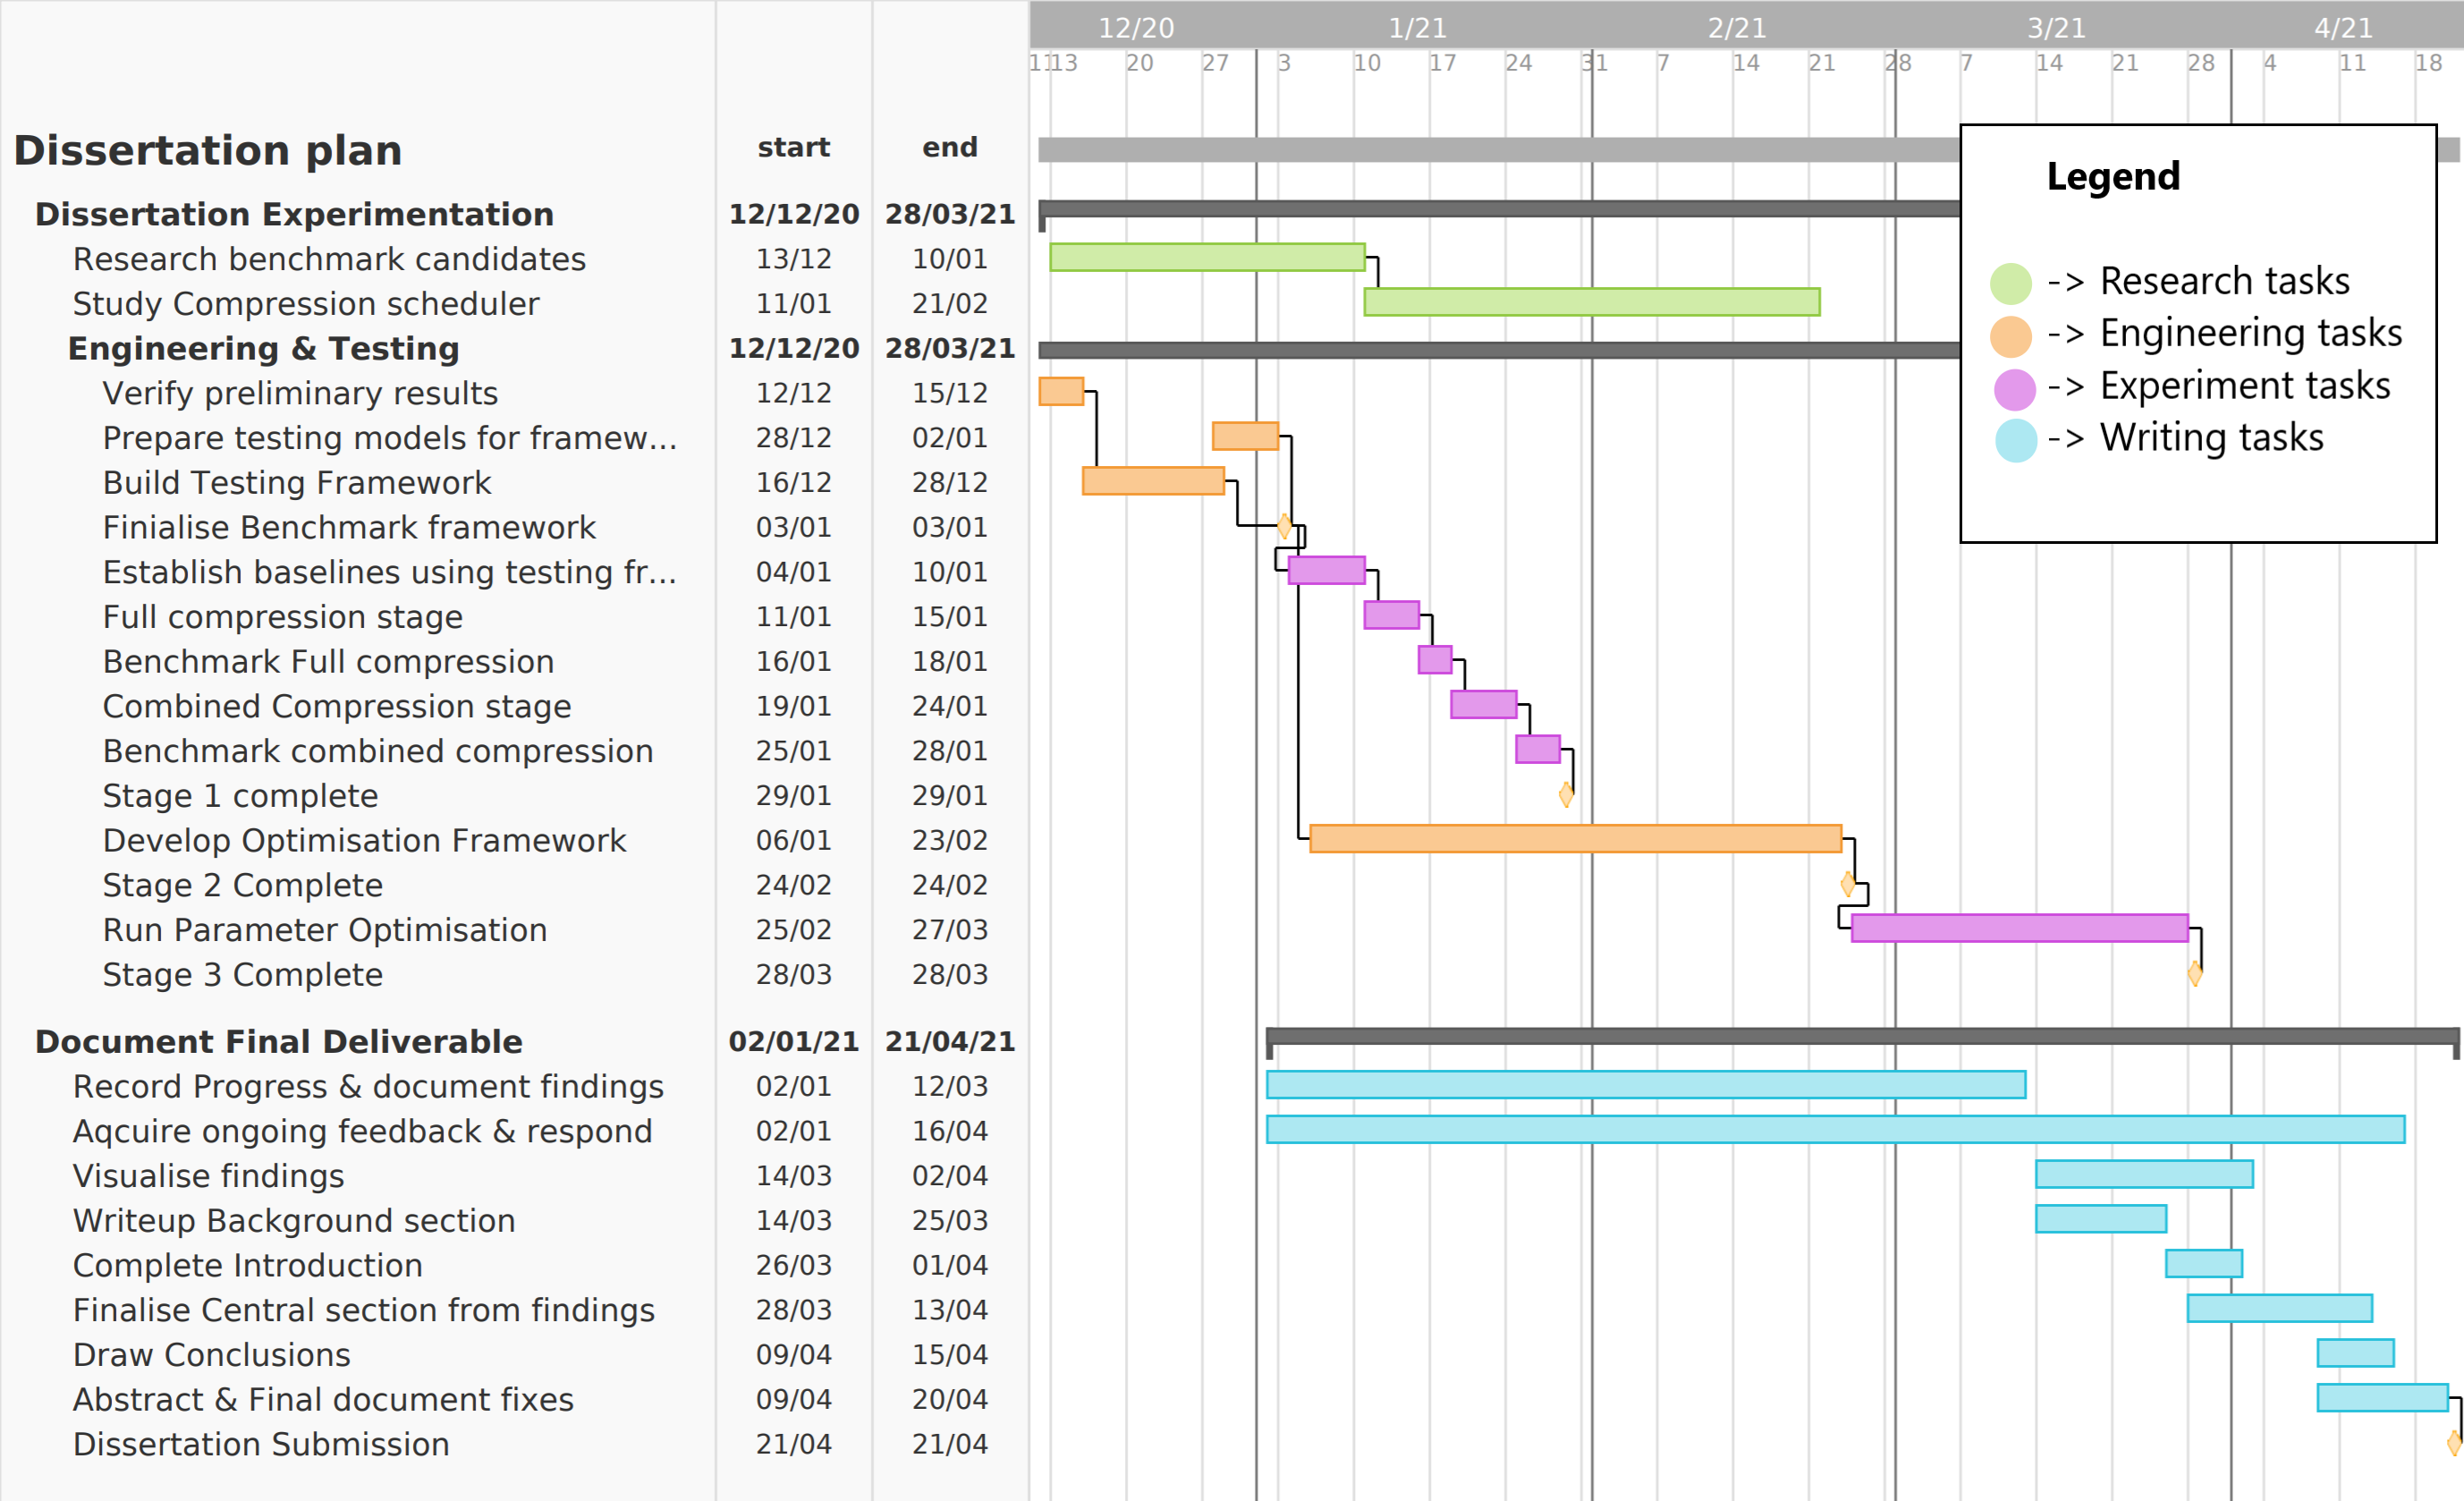
\includegraphics[width=1\textwidth]{GanttChart_legend.png}
    \caption{Project gantt chart}
    \label{fig:ganttChart}
\end{figure}

\subsection{Risk Analysis}
The following displays the anticipated risks with their accompanying mitigation strategies.
\begin{enumerate}
    \item Cannot compress model in Distiller.
    \begin{itemize}
        \item Investigate alternative compression libraries.
    \end{itemize}

    \item Issues with ONNX compatability.
    \begin{itemize}
        \item Investigate alternative intermediate representations.
        \item Manually export Distiller model to PyTorch and then directly to OpenVINO.
    \end{itemize}

    \item Bottleneck on time to train models.
    \begin{itemize}
        \item Add additional local Training agents (see Section~\ref{sec:ERdiagram}).
        \item Scale the experimental model size down.
        \item Cloud training agents could be added.
    \end{itemize}

    \item Bottleneck on time to benchmark inference.
    \begin{itemize}
        \item Investigate acquisition of a second NCS.
    \end{itemize}

    \item Time management issues.
    \begin{itemize}
        \item Make use of the project plan to properly manage deadlines.
        \item Reduce development complexity (remove parallel training agents)
    \end{itemize}

    \item Complexity of parameterising compression algorithm too high.
    \begin{itemize}
        \item Reduce scope of complexity by removing layer selection from the programatic definition and using a static layer definition.
    \end{itemize}

    \item Illness
    \begin{itemize}
        \item Compensate for unexpected delays in the project plan
    \end{itemize}
\end{enumerate}


\begin{table}[]
    \begin{tabular}{@{}|l|l|l|l|l|l|l|@{}}
        \toprule
        \multirow{7}{*}{Likelihood} & Near Certainty $\sim$90\% &            &       &          &         &          \\ \cmidrule(l){2-7} 
                                    & Highly Likely $\sim$70\%  &            &       &          &         &          \\ \cmidrule(l){2-7} 
                                    & Likely $\sim$50\%         &            &       &          &         &          \\ \cmidrule(l){2-7} 
                                    & Low likelihood $\sim$30\% &            &       &          &         &          \\ \cmidrule(l){2-7} 
                                    & Not Likely $\sim$10\%     &            &       &          &         &          \\ \cmidrule(l){2-7} 
                                    & \multirow{2}{*}{}         & Negligible & Minor & Moderate & Serious & Critical \\ \cmidrule(l){3-7} 
                                    &                           & \multicolumn{5}{l|}{Impact of unmitigated Risk}  \\ \bottomrule
        \end{tabular}
    \caption{Unmitigated risk trace}
\end{table}




\subsection{Professional, Legal, Ethical, \& Social issues}
This dissertation will not use any participants in any experiments so there are no ethical or legal issues concerning the safety or well being of participants.


Care will be taken during the course of this dissertaion to maintain a professional standard of communication regarding this work with all contemporaries. 


All software produced in the course of this work will be open source and licensed under the Apache License 2.0, this is in  compliance with the existing Apache License 2.0 that is already in place on the Distiller and OpenVINO repositories if any modifications are made to the software of those respective libraries.
Redis is licensed under the BSD license, Weights and Biases provides a free academic and open source license, this has been applied for and acquired.


The broader technological and social issues that this work may or may not play a part in are unknown, the field of machine learning is advancing at a tremendous pace (at the time of writing), and while it is vital to consider these implications they go far beyond the scope of this work. 
Any impact this dissertation will be just a miniscule part of a much larger technological revolution in which very few (if any) understand the full depth of the implications of their individual contributions.

\end{document}